\documentclass[a4paper,12pt]{scrartcl}

\usepackage{bm,amsmath,url,graphicx}
\usepackage{palatino}
\usepackage{color, xcolor}
\usepackage{listings}


\newcommand{\n}{\mathbf{ n}}
\newcommand{\h}{\mathbf{ h}}
\newcommand{\x}{\mathbf{ x}}
\newcommand{\y}{\mathbf{ y}}
\newcommand{\w}{\mathbf{ w}}
\newcommand{\HH}{\mathbf{ H}}
\newcommand{\R}{\mathbf{ R}}
\newcommand{\C}{\mathbf{ C}}
\newcommand{\thb}{{\boldsymbol{\theta}}}
\newcommand{\mub}{{\boldsymbol{\mu}}}
\newcommand{\python}{{\fbox{\texttt{\bfseries python}}\quad}}
\newcommand{\pen}{{\fbox{\texttt{\bfseries pen\&paper}}\quad}}

\renewcommand{\familydefault}{\rmdefault}


\begin{document}
\section*{SGN-41007 Pattern Recognition and Machine Learning}
\emph{Exercise Set 6: February 15--February 17, 2017}
\bigskip
\sloppy

\lstdefinestyle{mystyle}{
  belowcaptionskip=1\baselineskip,
  breaklines=true,
  frame=single,
  xleftmargin=\parindent,
  language=Python,
  showstringspaces=false,
  basicstyle=\ttfamily,
  keywordstyle=\bfseries\color{green!40!black},
  commentstyle=\itshape\color{purple!40!black},
  identifierstyle=\color{blue},
  stringstyle=\color{orange},
  moredelim=**[is][\color{red}]{@}{@},
}

\lstset{language=Python,style=mystyle} 


\noindent
Exercises consist of both pen\&paper and computer assignments.
Pen\&paper questions are solved at home before exercises, while
computer assignments are solved during exercise hours. The
computer assignments are marked by  \python and 
Pen\&paper questions by  \pen
\medskip

\noindent\textbf{Note: Python exercises can not be executed in Pinni ML1084.
Try to bring your own laptop with Anaconda installed. We will form 
groups around those machines that have Keras.}

\begin{enumerate}

\item \pen \emph{Derive an estimate for the variance of the random forest.}

The efficiency of the random forest relies on the variability of the
individual weak trees. However, this results in randomness of the
results, as well: If you run training 10 times, you may have 10
different results.

Increasing the number of trees helps to reduce the variation of outputs,
as seen in Figure~\ref{fig:variances}. More trees mean less variation.
However, the question remains: how many trees is enough.

The number of trees can be assessed theoretically via the following
theorem in a regression context (output of the RF is the average of
individual trees).

Consider the prediction of trees $1,2,\ldots, N$ as random variables
$T_1, T_2,\ldots, T_N$, each with identical variance $\sigma^2$. 
If the predictions were independent, their average would have variance
$\sigma^2/N$. However, if the RV's have pairwise correlation coefficient
$\rho$, show that the variance of the average is given as
\[
\rho\sigma^2 + \frac{1-\rho}{N}\sigma^2
\]


\begin{figure}[b]%
\centerline{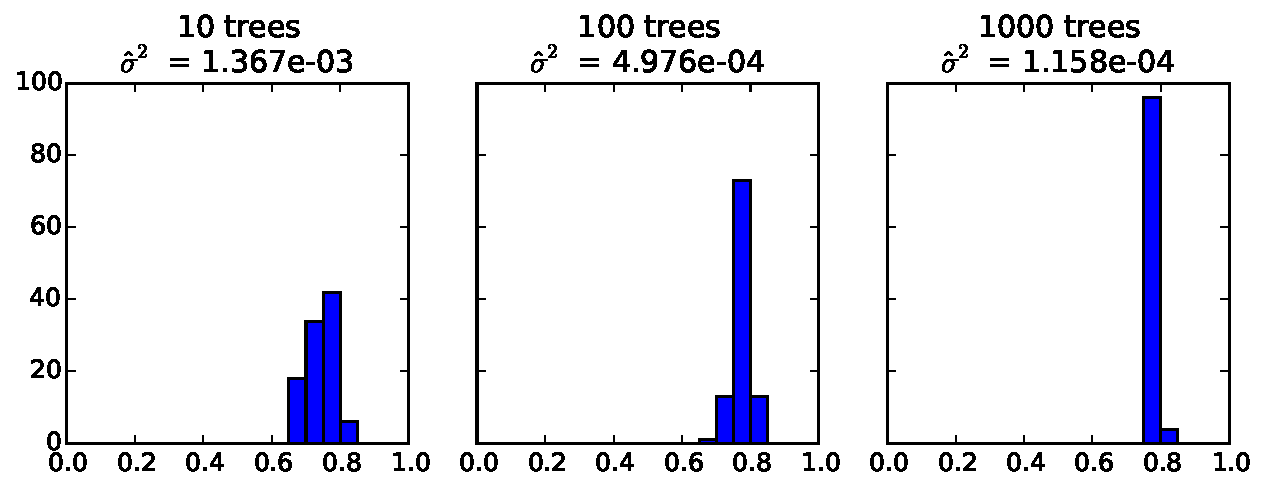
\includegraphics[width=0.6\columnwidth]{Variances.pdf}}%
\caption{Variances of random forest with different number of trees.}%
\label{fig:variances}%
\end{figure}

\eject

\item \pen {Count the number of parameters in a neural network}

Consider the traditional shallow neural network architecture 
of Figure~\ref{fig:net}. Suppose our inputs are $64\times 64$
bitmaps of two categories of traffic signs.
\begin{enumerate}
\item Let the network structure be the following:
\begin{itemize}
	\item The input is $3\times 64\times 64 = 12288$-dimensional
	\item On the 1st layer there are 100 nodes (marked in blue)
	\item On the 2nd layer there are 100 nodes (marked in blue)
	\item On the 3rd (output) layer there are 10 nodes (marked in blue; one for each class)
\end{itemize}
Compute the number of parameters (coefficients) in the net.

\item Consider the following code defining a convolutional architecture 
and compute the number of coefficients in this case.
\begin{lstlisting}
N = 10        # Number of feature maps
w, h = 3, 3   # Conv. window size

model = Sequential()

model.add(Convolution2D(nb_filter = N,
                        nb_col = w,
                        nb_row = h,
                        activation = 'relu',
                        border_mode = 'same',
                        input_shape = (3,64,64)))												
model.add(MaxPooling2D((2,2)))

model.add(Convolution2D(nb_filter = N,
                        nb_col = w,
                        nb_row = h,
                        border_mode = 'same',
                        activation = 'relu'))												
model.add(MaxPooling2D((2,2)))  

model.add(Flatten())
model.add(Dense(2, activation = 'sigmoid'))
\end{lstlisting}

\item An old rule of thumb states that the number of training samples should be at least 
5 times the number of coefficients. Compute the desired sample size based on this rule for (a) and (b).
\end{enumerate}


\begin{figure}%
\centerline{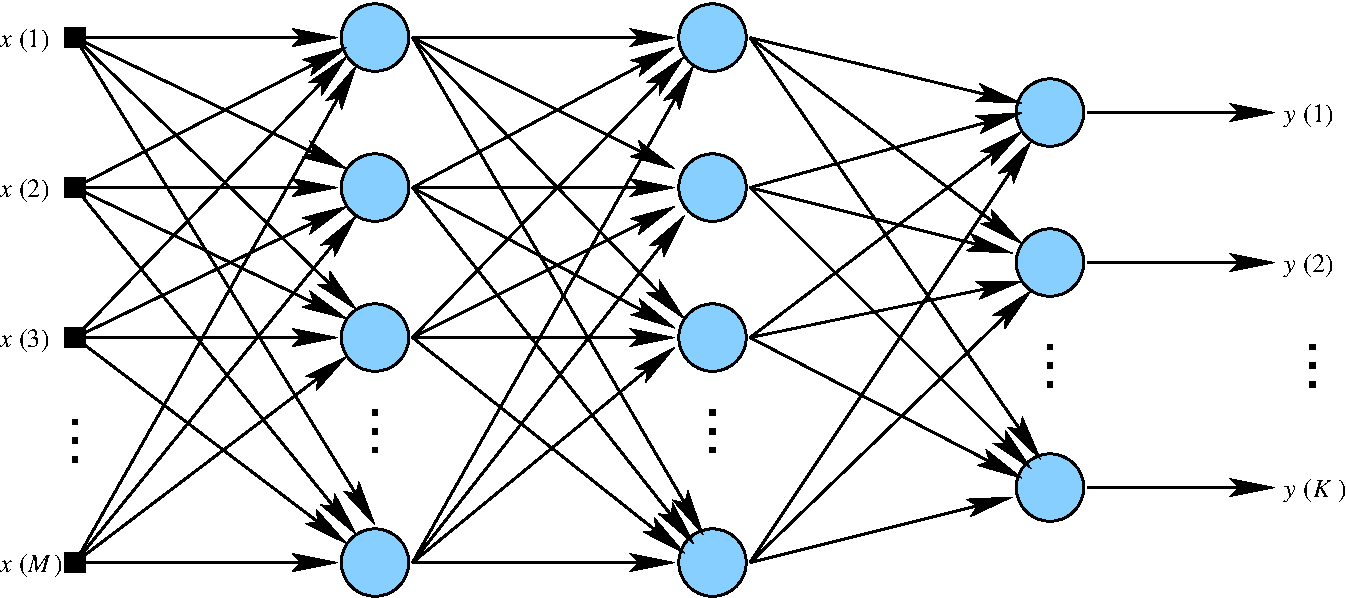
\includegraphics[width=0.6\columnwidth]{VanillaNeuralNet.pdf}}%
\caption{Vanilla neural network.}%
\label{fig:net}%
\end{figure}

\item \python \emph{Load Traffic sign data for deep neural network processing.}

Download an extended version of the two class German Traffic Sign
Recognition Benchmark (GTSRB) dataset from 

\url{http://www.cs.tut.fi/courses/SGN-41006/GTSRB_subset_2.zip}

This time, images are in color and there are about 400 from both classes.
Edit your previous script (exercise set 4) such that the image array will
have dimension (660, 3, 64, 64): 660 images of size 64x64 and 3 color channels.
You will need \verb+numpy.transpose+ to reorder dimensions: (64, 64, 3) $\rightarrow$ (3, 64, 64).

After collecting the data, normalize all samples into range [0,1];
\emph{i.e.,} subtract \verb+numpy.min(X)+ and divide the result
by \verb+numpy.max(X)+. Make sure that you are using float (not integer)
division.

Finally, split the data to training and testing (80\% / 20\%)
using \verb+sklearn.cross_validation.train_test_split+.

\item \python \emph{Define the network in Keras.}

Define the network of Question 2b in your code.

\item \python \emph{Compile and train the net.}

\textbf{Note:} You need to set up Keras to use the Theano backend instead of
Tensorflow (the default). To this aim, your config file \verb+~/.keras/keras.json+
has to look like this:
\begin{verbatim}
{
    "image_dim_ordering": "th", 
    "epsilon": 1e-07, 
    "floatx": "float32", 
    "backend": "theano",
    "optimizer": "None"
}
\end{verbatim}

Compile and train the network as described in 

\url{https://keras.io/models/sequential/}

Use the following parameters:
\begin{itemize}
	\item \textbf{Loss:} binary crossentropy (same thing as log loss; see previous exercises)
	\item \textbf{Optimizer:} stochastic gradient descent
	\item \textbf{Minibatch size:} 32
	\item \textbf{Number of epochs:} 20
\end{itemize}
Also add the parameter \verb+metrics=['accuracy']+ as an argument of
\verb+model.compile+ and give the test data to training algorithm
\verb+model.fit(..., validation_data = [X_test, y_test])+
Then, the optimizer will report the test error every epoch.
\end{enumerate}

\end{document}          
